\documentclass[aspectratio=169]{beamer}

% Shared preamble for Claude Code slide decks
% Usage: % Shared preamble for Claude Code slide decks
% Usage: % Shared preamble for Claude Code slide decks
% Usage: \input{preamble} after \documentclass[aspectratio=169]{beamer}

\usetheme{default}
\usecolortheme{dove}

\setbeamertemplate{navigation symbols}{}
\setbeamertemplate{footline}{%
  \hfill{\large\insertframenumber\,/\,\inserttotalframenumber}\hspace{0.8em}\vspace{0.5em}%
}

\definecolor{popblue}{RGB}{52, 101, 164}
\definecolor{sampred}{RGB}{204, 0, 0}
\definecolor{paramgreen}{RGB}{0, 140, 70}
\definecolor{lightbg}{RGB}{245, 245, 250}
\definecolor{warnred}{RGB}{180, 40, 40}
\definecolor{orange1}{RGB}{220, 120, 0}
\definecolor{violet1}{RGB}{120, 50, 160}

\setbeamercolor{frametitle}{fg=popblue}
\setbeamercolor{title}{fg=popblue}
\setbeamercolor{block title}{fg=white,bg=popblue}
\setbeamercolor{block body}{bg=lightbg}
\setbeamercolor{block title alerted}{fg=white,bg=warnred}
\setbeamercolor{block body alerted}{bg=lightbg}
\setbeamercolor{block title example}{fg=white,bg=paramgreen}
\setbeamercolor{block body example}{bg=lightbg}

\usepackage{listings}
\usepackage[T1]{fontenc}
\usepackage{hyperref}
\usepackage{tikz}
\usepackage{booktabs}
\usetikzlibrary{shapes, arrows.meta, positioning, calc}

\lstset{
  basicstyle=\ttfamily\scriptsize,
  keywordstyle=\color{popblue}\bfseries,
  stringstyle=\color{paramgreen},
  commentstyle=\color{gray},
  breaklines=true,
  frame=single,
  backgroundcolor=\color{lightbg},
  rulecolor=\color{popblue!30},
  showstringspaces=false,
  columns=fullflexible,
}
 after \documentclass[aspectratio=169]{beamer}

\usetheme{default}
\usecolortheme{dove}

\setbeamertemplate{navigation symbols}{}
\setbeamertemplate{footline}{%
  \hfill{\large\insertframenumber\,/\,\inserttotalframenumber}\hspace{0.8em}\vspace{0.5em}%
}

\definecolor{popblue}{RGB}{52, 101, 164}
\definecolor{sampred}{RGB}{204, 0, 0}
\definecolor{paramgreen}{RGB}{0, 140, 70}
\definecolor{lightbg}{RGB}{245, 245, 250}
\definecolor{warnred}{RGB}{180, 40, 40}
\definecolor{orange1}{RGB}{220, 120, 0}
\definecolor{violet1}{RGB}{120, 50, 160}

\setbeamercolor{frametitle}{fg=popblue}
\setbeamercolor{title}{fg=popblue}
\setbeamercolor{block title}{fg=white,bg=popblue}
\setbeamercolor{block body}{bg=lightbg}
\setbeamercolor{block title alerted}{fg=white,bg=warnred}
\setbeamercolor{block body alerted}{bg=lightbg}
\setbeamercolor{block title example}{fg=white,bg=paramgreen}
\setbeamercolor{block body example}{bg=lightbg}

\usepackage{listings}
\usepackage[T1]{fontenc}
\usepackage{hyperref}
\usepackage{tikz}
\usepackage{booktabs}
\usetikzlibrary{shapes, arrows.meta, positioning, calc}

\lstset{
  basicstyle=\ttfamily\scriptsize,
  keywordstyle=\color{popblue}\bfseries,
  stringstyle=\color{paramgreen},
  commentstyle=\color{gray},
  breaklines=true,
  frame=single,
  backgroundcolor=\color{lightbg},
  rulecolor=\color{popblue!30},
  showstringspaces=false,
  columns=fullflexible,
}
 after \documentclass[aspectratio=169]{beamer}

\usetheme{default}
\usecolortheme{dove}

\setbeamertemplate{navigation symbols}{}
\setbeamertemplate{footline}{%
  \hfill{\large\insertframenumber\,/\,\inserttotalframenumber}\hspace{0.8em}\vspace{0.5em}%
}

\definecolor{popblue}{RGB}{52, 101, 164}
\definecolor{sampred}{RGB}{204, 0, 0}
\definecolor{paramgreen}{RGB}{0, 140, 70}
\definecolor{lightbg}{RGB}{245, 245, 250}
\definecolor{warnred}{RGB}{180, 40, 40}
\definecolor{orange1}{RGB}{220, 120, 0}
\definecolor{violet1}{RGB}{120, 50, 160}

\setbeamercolor{frametitle}{fg=popblue}
\setbeamercolor{title}{fg=popblue}
\setbeamercolor{block title}{fg=white,bg=popblue}
\setbeamercolor{block body}{bg=lightbg}
\setbeamercolor{block title alerted}{fg=white,bg=warnred}
\setbeamercolor{block body alerted}{bg=lightbg}
\setbeamercolor{block title example}{fg=white,bg=paramgreen}
\setbeamercolor{block body example}{bg=lightbg}

\usepackage{listings}
\usepackage[T1]{fontenc}
\usepackage{hyperref}
\usepackage{tikz}
\usepackage{booktabs}
\usetikzlibrary{shapes, arrows.meta, positioning, calc}

\lstset{
  basicstyle=\ttfamily\scriptsize,
  keywordstyle=\color{popblue}\bfseries,
  stringstyle=\color{paramgreen},
  commentstyle=\color{gray},
  breaklines=true,
  frame=single,
  backgroundcolor=\color{lightbg},
  rulecolor=\color{popblue!30},
  showstringspaces=false,
  columns=fullflexible,
}


\title{AI Tools for Learning \& Education}
\subtitle{How to use LLMs and AI tools to learn better, not less}
\author{Hayk Tarkhanyan}
\date{}

\begin{document}

% ──────────────────────────────────────────────
\begin{frame}
\titlepage
\end{frame}

% ──────────────────────────────────────────────
\begin{frame}{The AI Education Explosion}

\begin{center}
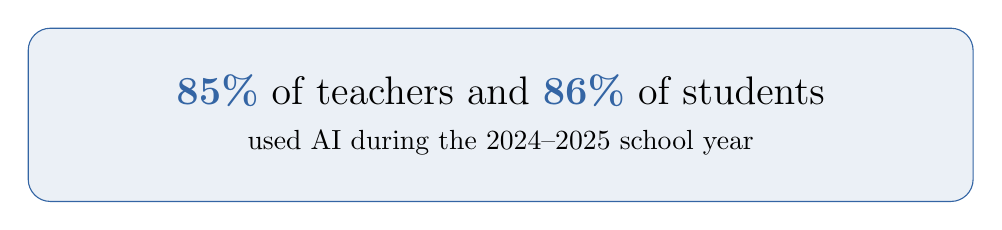
\begin{tikzpicture}
  \node[draw=popblue, fill=popblue!10, rounded corners=8pt,
        minimum width=12cm, minimum height=2.2cm, align=center] {
    {\Large \textbf{\color{popblue}85\%} of teachers and
     \textbf{\color{popblue}86\%} of students}\\[4pt]
    used AI during the 2024--2025 school year
  };
\end{tikzpicture}
\end{center}

\bigskip
All three major LLMs launched education-specific modes within weeks of each other:

\begin{columns}[T]
\column{0.33\textwidth}
\begin{center}
\textbf{\color{popblue}ChatGPT}\\Study Mode\\{\small July 2025}
\end{center}

\column{0.33\textwidth}
\begin{center}
\textbf{\color{violet1}Claude}\\Learning Mode\\{\small August 2025}
\end{center}

\column{0.33\textwidth}
\begin{center}
\textbf{\color{paramgreen}Gemini}\\Guided Learning\\{\small August 2025}
\end{center}
\end{columns}

\bigskip
\begin{center}
The question isn't \emph{whether} to use AI --- it's \textbf{how to use it well}.
\end{center}
\end{frame}

% ──────────────────────────────────────────────
\begin{frame}{The Core Tension}

\begin{center}
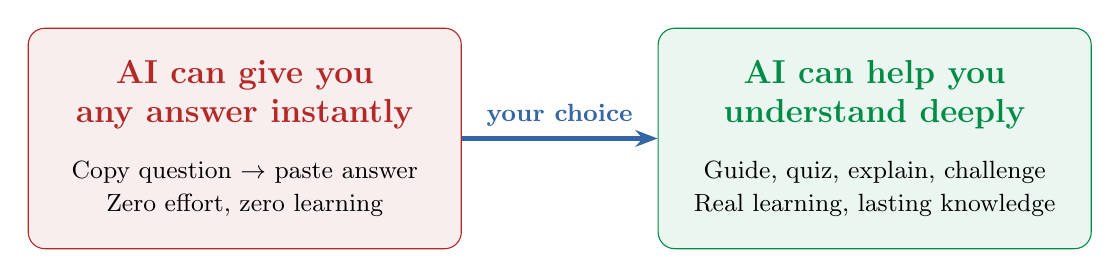
\begin{tikzpicture}
  % Left box: the temptation
  \node[draw=warnred, fill=warnred!8, rounded corners=6pt,
        minimum width=5.5cm, minimum height=2.8cm, align=center]
        (bad) at (-4,0) {
    {\large \color{warnred}\textbf{AI can give you}}\\[2pt]
    {\large \color{warnred}\textbf{any answer instantly}}\\[8pt]
    {\small Copy question $\to$ paste answer}\\
    {\small Zero effort, zero learning}
  };

  % Right box: the opportunity
  \node[draw=paramgreen, fill=paramgreen!8, rounded corners=6pt,
        minimum width=5.5cm, minimum height=2.8cm, align=center]
        (good) at (4,0) {
    {\large \color{paramgreen}\textbf{AI can help you}}\\[2pt]
    {\large \color{paramgreen}\textbf{understand deeply}}\\[8pt]
    {\small Guide, quiz, explain, challenge}\\
    {\small Real learning, lasting knowledge}
  };

  % Arrow
  \draw[-{Stealth[length=8pt]}, line width=2pt, popblue]
    (bad.east) -- node[above, font=\small\bfseries] {your choice} (good.west);
\end{tikzpicture}
\end{center}

\bigskip
\begin{center}
\textit{``AI should make students think harder, not less.''} --- Anthropic
\end{center}
\end{frame}

% ──────────────────────────────────────────────
\begin{frame}{What We'll Cover}

\begin{columns}[T]
\column{0.25\textwidth}
\textbf{\color{popblue}1. The Big Three}
\begin{itemize}
  \item ChatGPT Study Mode
  \item Claude Learning Mode
  \item Gemini Guided Learning
  \item Side-by-side comparison
\end{itemize}

\column{0.25\textwidth}
\textbf{\color{paramgreen}2. Specialized Tools}
\begin{itemize}
  \item NotebookLM
  \item Perplexity AI
  \item Khanmigo
  \item Math, coding, writing tools
\end{itemize}

\column{0.25\textwidth}
\textbf{\color{orange1}3. How to Learn}
\begin{itemize}
  \item The right way vs.\ wrong way
  \item Prompting for learning
  \item Study session workflow
\end{itemize}

\column{0.25\textwidth}
\textbf{\color{violet1}4. Pitfalls \& Tips}
\begin{itemize}
  \item Hallucinations
  \item Academic integrity
  \item Privacy \& data
  \item Free access guide
\end{itemize}
\end{columns}
\end{frame}

% ══════════════════════════════════════════════
% SECTION 2: The Big Three LLMs
% ══════════════════════════════════════════════
\section{The Big Three LLMs --- Education Modes}

% ──────────────────────────────────────────────
\begin{frame}{ChatGPT Study Mode}

\textbf{\color{popblue}Launched:} July 2025 \quad|\quad
\textbf{\color{popblue}Access:} Free tier (select ``study and learn'' in tools)

\bigskip
\begin{columns}[T]
\column{0.55\textwidth}
\textbf{How it works:}
\begin{itemize}
  \item Guides you step-by-step instead of giving answers
  \item \textbf{Refuses} direct answers until you engage with the material
  \item Asks questions to test your understanding
  \item Calibrates to your skill level
\end{itemize}

\bigskip
\textbf{Interactive Learning:}
\begin{itemize}
  \item 70+ math \& science topics
  \item Pythagorean theorem, ideal gas law, lens equations\ldots
  \item Visualizations for complex concepts
\end{itemize}

\column{0.42\textwidth}
\begin{block}{Example interaction}
\ttfamily\scriptsize
\textbf{You:} How do I find the derivative\\
of $f(x) = x^3 + 2x$?\\[4pt]
\textbf{ChatGPT:} Before I show you,\\
let me ask --- do you remember\\
the power rule? What happens\\
when you differentiate $x^n$?\\[4pt]
\textbf{You:} $nx^{n-1}$?\\[4pt]
\textbf{ChatGPT:} Exactly! Now try\\
applying that to each term\ldots
\end{block}
\end{columns}
\end{frame}

% ──────────────────────────────────────────────
\begin{frame}{ChatGPT Study Mode: Features}
\small
\begin{columns}[T]
\column{0.48\textwidth}
\begin{exampleblock}{Upcoming features}
\begin{itemize}\setlength\itemsep{0em}
  \item Clearer visualizations for complex concepts
  \item Goal setting \& progress tracking
  \item Deeper personalization by skill level
\end{itemize}
\end{exampleblock}

\smallskip
\textbf{\color{popblue}Also useful for learning:}
\begin{itemize}\setlength\itemsep{0em}
  \item \textbf{Canvas} --- side-by-side editing for writing/code
  \item \textbf{Memory} --- remembers your course, level, preferences
  \item \textbf{Custom GPTs} --- course-specific chatbots
  \item \textbf{Voice mode} --- conversational tutoring
  \item \textbf{File upload} --- problem sets, diagrams, documents
\end{itemize}

\column{0.48\textwidth}
\begin{alertblock}{Demo idea}
Open ChatGPT $\to$ ``study and learn'' $\to$ try a math problem. Notice how it guides rather than solves.
\end{alertblock}

\smallskip
\textbf{\color{popblue}ChatGPT Edu:}
\begin{itemize}\setlength\itemsep{0em}
  \item Dedicated tier for universities
  \item GPT-4o access, enterprise-grade privacy
  \item Admin controls, SSO, group workspaces
\end{itemize}
\end{columns}
\end{frame}

% ──────────────────────────────────────────────
\begin{frame}{Claude: Learning \& Explanatory Modes}

\textbf{\color{violet1}Launched:} August 2025 \quad|\quad
\textbf{\color{violet1}Stat:} 76\% of users reported improved understanding

\bigskip
\begin{columns}[T]
\column{0.48\textwidth}
\begin{block}{Learning Mode}
\textbf{Socratic pair-programming}
\begin{itemize}
  \item Pauses and inserts \texttt{\#TODO} for you to write code
  \item You complete 5--10 lines yourself
  \item Claude reviews your work and guides further
  \item Learn by doing, not by reading
\end{itemize}
\end{block}

\column{0.48\textwidth}
\begin{block}{Explanatory Mode}
\textbf{Senior dev mentoring}
\begin{itemize}
  \item Narrates every decision as it works
  \item Explains architecture choices, tradeoffs
  \item Shares best practices in real-time
  \item Like looking ``under the hood''
\end{itemize}
\end{block}
\end{columns}

\bigskip
\textbf{\color{violet1}Claude for Education} (since April 2025):
deployed at Northeastern (50K users), LSE, Champlain College.
\textit{``AI should make students think harder, not less.''}
\end{frame}

% ──────────────────────────────────────────────
\begin{frame}{Claude: Example Interaction}

\begin{columns}[T]
\column{0.48\textwidth}
\begin{block}{Learning Mode example}
\ttfamily\scriptsize
\textbf{You:} Help me write a function\\
that reverses a linked list.\\[4pt]
\textbf{Claude:} Let's build this together.\\
I'll set up the structure ---\\
you write the core logic.\\[4pt]
def reverse\_list(head):\\
\quad prev = None\\
\quad current = head\\
\quad \# TODO: Write a while loop that\\
\quad \# iterates through the list and\\
\quad \# reverses the pointers.\\
\quad \# (about 5 lines)\\
\quad return prev
\end{block}

\column{0.48\textwidth}
\begin{block}{Explanatory Mode example}
\ttfamily\scriptsize
\textbf{You:} Explain binary search.\\[4pt]
\textbf{Claude:} Binary search works on\\
\textbf{sorted} arrays. The key insight\\
is: by checking the middle element,\\
we eliminate \textbf{half} the remaining\\
candidates each step.\\[4pt]
Why sorted? Because if arr[mid]\\
is too large, everything to its\\
right is also too large. This\\
guarantee is what makes the\\
O(log n) complexity possible.\\[4pt]
Think of it like a phone book\ldots
\end{block}
\end{columns}

\bigskip
\begin{center}
\small\color{violet1}
Demo: Ask Claude to teach you a concept in Learning or Explanatory mode
\end{center}
\end{frame}

% ──────────────────────────────────────────────
\begin{frame}{Gemini Guided Learning}
\small
\textbf{\color{paramgreen}Launched:} August 2025 \quad|\quad
\textbf{\color{paramgreen}Built on:} LearnLM --- Google's education-specific AI

\smallskip
\begin{columns}[T]
\column{0.55\textwidth}
\textbf{How it works:}
\begin{itemize}\setlength\itemsep{0em}
  \item Socratic method + step-by-step guidance
  \item Won't just give you answers
  \item Asks questions to ensure you learned the concept
  \item LearnLM integrated into Gemini 2.5
\end{itemize}

\smallskip
\textbf{Key features:}
\begin{itemize}\setlength\itemsep{0em}
  \item \textbf{Canvas quizzes} --- personalized quizzes for any subject
  \item \textbf{Video Overviews} --- turn sources into educational videos
  \item \textbf{SAT prep} --- free practice tests (Princeton Review)
  \item Free for educational institutions
\end{itemize}

\column{0.42\textwidth}
\begin{exampleblock}{LearnLM stats}
\begin{itemize}\setlength\itemsep{0em}
  \item Only \textbf{0.1\%} factual error rate
  \item Students \textbf{5.5 pp} more likely to solve novel problems
  \item Preferred by educators over competitors
\end{itemize}
\end{exampleblock}

\smallskip
\begin{alertblock}{Demo idea}
Open Gemini $\to$ Guided Learning $\to$ ask about a concept. Notice the Socratic style.
\end{alertblock}
\end{columns}
\end{frame}

% ──────────────────────────────────────────────
\begin{frame}{Gemini: More Education Features}

\begin{columns}[T]
\column{0.48\textwidth}
\textbf{\color{paramgreen}Gemini for Students:}
\begin{itemize}
  \item Integration with Google Classroom, Docs, Slides
  \item Ask questions while reading documents
  \item Get help with assignments
  \item Research topics within your workflow
\end{itemize}

\bigskip
\textbf{\color{paramgreen}For teachers:}
\begin{itemize}
  \item Draft assignments in Classroom
  \item Summarize student progress
  \item Record/attach audio \& video for feedback
\end{itemize}

\column{0.48\textwidth}
\begin{block}{Example interaction}
\ttfamily\scriptsize
\textbf{You:} What causes ocean tides?\\[4pt]
\textbf{Gemini:} Good question! Before I\\
explain, let me check what you\\
already know. Can you think of\\
what celestial body might have the\\
biggest influence on tides?\\[4pt]
\textbf{You:} The moon?\\[4pt]
\textbf{Gemini:} Right! Now, why do you\\
think the moon specifically?\\
What property does it have that\\
could affect Earth's oceans?
\end{block}
\end{columns}
\end{frame}

% ──────────────────────────────────────────────
\begin{frame}{Side-by-Side Comparison}

\begin{center}
\small
\begin{tabular}{@{}l p{3.5cm} p{3.5cm} p{3.5cm}@{}}
\toprule
& \textbf{\color{popblue}ChatGPT} & \textbf{\color{violet1}Claude} & \textbf{\color{paramgreen}Gemini} \\
\midrule
\textbf{Mode name} & Study Mode & Learning / Explanatory & Guided Learning \\[4pt]
\textbf{Approach} & Refuses answers, quizzes & Socratic + \texttt{\#TODO} inserts & Socratic questioning \\[4pt]
\textbf{Best for} & Math/science, general study & Coding, technical concepts & Google ecosystem, quizzes \\[4pt]
\textbf{Unique} & 70+ interactive topics & Pair-programming style & LearnLM, Video Overviews \\[4pt]
\textbf{Free tier} & Yes & Yes & Yes (free for edu) \\[4pt]
\textbf{Ecosystem} & Canvas, Custom GPTs & Artifacts, Projects & Classroom, Docs, Slides \\
\bottomrule
\end{tabular}
\end{center}

\bigskip
\begin{center}
\textbf{Key insight:} all three are designed to \textbf{guide}, not \textbf{give answers}.\\
Try the same question in all three --- you'll notice different tutoring styles.
\end{center}
\end{frame}

% ──────────────────────────────────────────────
\begin{frame}{Same Question, Three Styles}

\textbf{Question:} \textit{``Explain how recursion works in programming.''}

\bigskip
\begin{columns}[T]
\column{0.32\textwidth}
\begin{block}{\color{popblue}ChatGPT Study Mode}
\scriptsize
\textit{Before I explain, tell me: have you heard of a function calling itself? What do you think would happen if a function called itself without stopping?}

\medskip
$\to$ Tests your understanding first
\end{block}

\column{0.32\textwidth}
\begin{block}{\color{violet1}Claude Learning Mode}
\scriptsize
\textit{Let's learn by building. Here's a skeleton for factorial:}

\texttt{def factorial(n):}\\
\texttt{\quad \# TODO: Write the base}\\
\texttt{\quad \# case and recursive call}

\medskip
$\to$ Makes you write the code
\end{block}

\column{0.32\textwidth}
\begin{block}{\color{paramgreen}Gemini Guided}
\scriptsize
\textit{Great topic! Think of Russian nesting dolls --- each doll contains a smaller one. What would be the ``smallest doll'' in a recursive function?}

\medskip
$\to$ Uses analogies, then guides
\end{block}
\end{columns}

\bigskip
\begin{center}
\small\color{orange1}
Optional demo: ask the same question to all three and compare live
\end{center}
\end{frame}

% ══════════════════════════════════════════════
% SECTION 3: Specialized AI Tools
% ══════════════════════════════════════════════
\section{Specialized AI Tools}

% ──────────────────────────────────────────────
\begin{frame}{NotebookLM: Your Personal Study Assistant}
\small
\textbf{\color{popblue}What:} Upload YOUR materials $\to$ AI assistant grounded in YOUR sources

\smallskip
\begin{columns}[T]
\column{0.55\textwidth}
\textbf{How it's different from chatbots:}
\begin{itemize}\setlength\itemsep{0em}
  \item Regular LLMs answer from training data (generic internet)
  \item NotebookLM answers from \textbf{your uploaded documents}
  \item Source-grounded = fewer hallucinations
  \item Every answer references your materials
\end{itemize}

\smallskip
\textbf{What you can upload:}
\begin{itemize}\setlength\itemsep{0em}
  \item PDFs, Google Docs, Slides
  \item Lecture notes, textbook chapters
  \item Research papers, YouTube videos, audio
\end{itemize}

\column{0.42\textwidth}
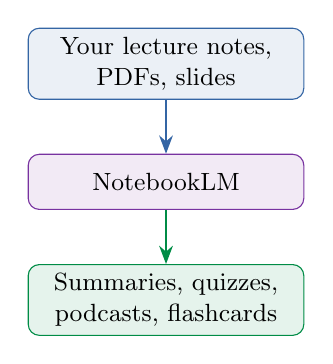
\begin{tikzpicture}[
  box/.style={draw=popblue, rounded corners=4pt, minimum width=3.5cm,
              minimum height=0.7cm, align=center, font=\small},
  arr/.style={-{Stealth}, thick, popblue}
]
  \node[box, fill=popblue!10] (src) at (0,3) {Your lecture notes,\\PDFs, slides};
  \node[box, fill=violet1!10, draw=violet1] (nlm) at (0,1.5) {NotebookLM};
  \node[box, fill=paramgreen!10, draw=paramgreen] (out) at (0,0) {Summaries, quizzes,\\podcasts, flashcards};
  \draw[arr] (src) -- (nlm);
  \draw[arr, paramgreen] (nlm) -- (out);
\end{tikzpicture}
\end{columns}
\end{frame}

% ──────────────────────────────────────────────
\begin{frame}{NotebookLM: Key Features}
\small
\begin{columns}[T]
\column{0.48\textwidth}
\begin{block}{Audio Overviews}
AI generates a \textbf{podcast-style discussion} of your materials. Two AI hosts discuss your content. Listen on commute, exercising, etc.
\end{block}

\smallskip
\begin{block}{Interactive Mode}
\textbf{``Raise your hand''} during the podcast. AI hosts stop, answer your question, then continue.
\end{block}

\column{0.48\textwidth}
\begin{block}{Flashcards \& Quizzes}
Auto-generated from your documents. Test yourself on \textbf{your actual course content}.
\end{block}

\smallskip
\begin{block}{Learning Guide}
Structured, deeper exploration of your materials. Beyond summaries --- builds understanding.
\end{block}

\smallskip
\begin{exampleblock}{Price}
\textbf{Free} for all education users.
\end{exampleblock}
\end{columns}

\smallskip
\begin{center}
\footnotesize\color{orange1}
Demo: upload a lecture PDF, generate an Audio Overview, try Interactive Mode
\end{center}
\end{frame}

% ──────────────────────────────────────────────
\begin{frame}{Perplexity AI: Research with Citations}
\small
\textbf{\color{popblue}What:} AI search engine --- every claim comes with a source

\smallskip
\begin{columns}[T]
\column{0.55\textwidth}
\textbf{Why it matters for students:}
\begin{itemize}\setlength\itemsep{0em}
  \item Unlike ChatGPT/Claude: \textbf{cites sources} for every claim
  \item Better than Google for research questions
  \item Synthesizes from multiple sources
  \item Academic-quality research in seconds
\end{itemize}

\smallskip
\textbf{Key features:}
\begin{itemize}\setlength\itemsep{0em}
  \item \textbf{Study Mode} --- flashcards, summaries, quizzes
  \item \textbf{Research Mode} --- in-depth academic analysis
  \item \textbf{Expanded Citations} --- up to 10$\times$ more sources
  \item Wiley partnership for academic content
\end{itemize}

\column{0.42\textwidth}
\begin{exampleblock}{Free Pro for students}
\begin{itemize}
  \item \textbf{12 months free} with edu email
  \item Referral program: earn up to 24 free months
  \item Includes all premium features
\end{itemize}
\end{exampleblock}

\smallskip
\begin{alertblock}{Caveat}
Best citation accuracy among AI search engines, but still \textbf{37\% error rate}. Always verify!
\end{alertblock}
\end{columns}

\smallskip
\begin{center}
\footnotesize\color{orange1}
Demo: compare Google search vs.\ Perplexity for a research question
\end{center}
\end{frame}

% ──────────────────────────────────────────────
\begin{frame}{Khanmigo: Purpose-Built AI Tutor}
\small
\textbf{\color{popblue}What:} Khan Academy's AI tutor --- designed for education from day one

\smallskip
\begin{columns}[T]
\column{0.55\textwidth}
\textbf{How it works:}
\begin{itemize}\setlength\itemsep{0em}
  \item Socratic method: guides, \textbf{never gives direct answers}
  \item Limitless patience --- guides until you get it
  \item Built on GPT-4, constrained for education
  \item Integrated with Khan Academy's content
\end{itemize}

\smallskip
\textbf{Features:}
\begin{itemize}\setlength\itemsep{0em}
  \item \textbf{Image upload} --- scan handwritten math
  \item Writing coach, debate partner
  \item Career coaching, speech support
\end{itemize}

\column{0.42\textwidth}
\begin{exampleblock}{Availability}
\begin{itemize}\setlength\itemsep{0em}
  \item \$4/month or \$44/year
  \item Free via many school districts
  \item 10+ languages: English, Spanish, Russian, Arabic, Hindi, Chinese\ldots
\end{itemize}
\end{exampleblock}

\smallskip
\textbf{\color{popblue}For teachers:}
\begin{itemize}\setlength\itemsep{0em}
  \item Standards-aligned lesson plans
  \item Student progress summaries
  \item Learning objectives, rubrics, quizzes
\end{itemize}
\end{columns}
\end{frame}

% ──────────────────────────────────────────────
\begin{frame}{Math \& Science Tools}
\small
\begin{columns}[T]
\column{0.32\textwidth}
\begin{block}{Wolfram Alpha}
\begin{itemize}\setlength\itemsep{0em}
  \item Computational knowledge engine
  \item Step-by-step solutions
  \item Advanced math, science, engineering
  \item Curated data + algorithms
  \item Gold standard for computation
\end{itemize}
\smallskip
{\footnotesize\color{paramgreen}\textbf{Best for:} advanced problems}
\end{block}

\column{0.32\textwidth}
\begin{block}{Photomath}
\begin{itemize}\setlength\itemsep{0em}
  \item Mobile app --- scan and solve
  \item Handwritten or printed math
  \item Instant step-by-step solutions
  \item Arithmetic through calculus
\end{itemize}
\smallskip
{\footnotesize\color{paramgreen}\textbf{Best for:} quick help on the go}
\end{block}

\column{0.32\textwidth}
\begin{block}{Symbolab}
\begin{itemize}\setlength\itemsep{0em}
  \item Step-by-step algebra \& calculus
  \item Practice problems with hints
  \item Interactive graphing
  \item Free tier available
\end{itemize}
\smallskip
{\footnotesize\color{paramgreen}\textbf{Best for:} learning step by step}
\end{block}
\end{columns}

\smallskip
\begin{center}
\small\textbf{Pro tip:} combine ChatGPT + Wolfram Alpha ---
ChatGPT guides the \emph{process}, Wolfram verifies the \emph{computation}.
\end{center}
\end{frame}

% ──────────────────────────────────────────────
\begin{frame}{AI for Writing \& Research}

\begin{columns}[T]
\column{0.32\textwidth}
\begin{block}{Grammarly AI}
\begin{itemize}
  \item Grammar, spelling, punctuation
  \item Style \& tone suggestions
  \item Plagiarism detection
  \item Works in browser, Word, Google Docs
  \item Free tier available
\end{itemize}
\medskip
{\small\color{paramgreen}\textbf{Best for:} polishing your writing}
\end{block}

\column{0.32\textwidth}
\begin{block}{Notion AI}
\begin{itemize}
  \item Organize notes \& knowledge
  \item Summarize long documents
  \item Generate content in your workspace
  \item Q\&A over your notes
  \item Student plan available
\end{itemize}
\medskip
{\small\color{paramgreen}\textbf{Best for:} organizing study materials}
\end{block}

\column{0.32\textwidth}
\begin{block}{Gamma AI}
\begin{itemize}
  \item AI presentation creation
  \item Text $\to$ beautiful slides in minutes
  \item No design skills needed
  \item Websites \& documents too
  \item Free tier available
\end{itemize}
\medskip
{\small\color{paramgreen}\textbf{Best for:} creating presentations fast}
\end{block}
\end{columns}
\end{frame}

% ──────────────────────────────────────────────
\begin{frame}{AI for Coding}
\small
\begin{columns}[T]
\column{0.48\textwidth}
\begin{block}{GitHub Copilot}
\begin{itemize}\setlength\itemsep{0em}
  \item AI pair programmer in your editor
  \item Code autocomplete + chat
  \item Explains code, suggests fixes
  \item \textbf{Free for students} (GitHub Education)
  \item Works in VS Code, JetBrains, etc.
\end{itemize}
\end{block}

\smallskip
\begin{block}{Replit AI}
\begin{itemize}\setlength\itemsep{0em}
  \item Browser-based coding environment
  \item AI assistance built in
  \item No setup needed --- great for beginners
\end{itemize}
\end{block}

\column{0.48\textwidth}
\begin{block}{Other coding assistants}
\begin{itemize}\setlength\itemsep{0em}
  \item \textbf{Claude Code} --- terminal-based AI agent
  \item \textbf{Cursor} --- AI-first code editor
  \item \textbf{AskCodi} --- debug \& explain (free)
  \item \textbf{ChatGPT / Claude / Gemini} --- paste code, ask questions
\end{itemize}
\end{block}

\smallskip
\begin{exampleblock}{Learning tip}
Don't just accept generated code. Use \textbf{Learning Mode} or ask: \textit{``Explain this code line by line.''}
\end{exampleblock}
\end{columns}
\end{frame}

% ──────────────────────────────────────────────
\begin{frame}{AI for Language Learning}
\small
\begin{columns}[T]
\column{0.48\textwidth}
\begin{block}{Dedicated tools}
\begin{itemize}\setlength\itemsep{0em}
  \item \textbf{Duolingo} --- gamified, AI-adaptive, roleplay conversations
  \item \textbf{Speak} --- AI conversation partner
  \item \textbf{ELSA Speak} --- pronunciation feedback
\end{itemize}
\end{block}

\smallskip
\textbf{\color{popblue}Why LLMs are game-changers:}
\begin{itemize}\setlength\itemsep{0em}
  \item Free-form conversation in any language
  \item Correct mistakes with explanations
  \item Adapt to your level automatically
  \item Available 24/7
\end{itemize}

\column{0.48\textwidth}
\begin{block}{Using LLMs for languages}
\begin{itemize}\setlength\itemsep{0em}
  \item \textbf{Voice modes} --- speak and listen
  \item Practice real conversations
  \item Grammar explanations in your language
  \item Role-play: ordering food, interviews\ldots
\end{itemize}
\end{block}

\smallskip
\begin{exampleblock}{Try this prompt}
\textit{``Let's talk in French. I'm B1. Correct my mistakes gently and explain why.''}
\end{exampleblock}
\end{columns}
\end{frame}

% ──────────────────────────────────────────────
\begin{frame}{The AI Learning Toolkit}

\begin{center}
\textbf{\color{popblue}\large What do you need? $\to$ Use this tool}
\end{center}

\bigskip
\begin{center}
\small
\begin{tabular}{@{}l l l@{}}
\toprule
\textbf{Task} & \textbf{Best Tool} & \textbf{Why} \\
\midrule
Research with sources & Perplexity AI & Citations for every claim \\[3pt]
Study from your notes & NotebookLM & Grounded in your materials \\[3pt]
Understand a concept & ChatGPT / Claude / Gemini & Learning/education modes \\[3pt]
Solve math step-by-step & Wolfram Alpha / Photomath & Computational accuracy \\[3pt]
Write code & GitHub Copilot / Claude & Free for students, explains code \\[3pt]
Improve your writing & Grammarly AI & Grammar, style, tone \\[3pt]
Create a presentation & Gamma AI & Text $\to$ slides in minutes \\[3pt]
Practice a language & Duolingo + LLM voice & Structured + free-form practice \\[3pt]
Organized note-taking & Notion AI & Summarize, search, generate \\
\bottomrule
\end{tabular}
\end{center}

\bigskip
\begin{center}
\textbf{Best results come from \textcolor{paramgreen}{combining tools}}, not relying on one.
\end{center}
\end{frame}

% ══════════════════════════════════════════════
% SECTION 4: How to Actually Learn with AI
% ══════════════════════════════════════════════
\section{How to Actually Learn with AI}

% ──────────────────────────────────────────────
\begin{frame}{The Wrong Way}

\begin{center}
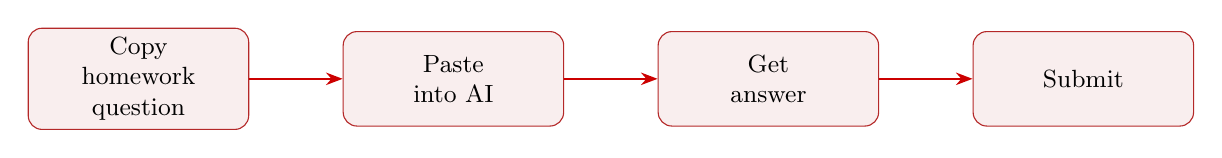
\begin{tikzpicture}[
  box/.style={draw=warnred, fill=warnred!8, rounded corners=5pt,
              minimum width=2.8cm, minimum height=1.2cm, align=center, font=\small},
  arr/.style={-{Stealth[length=6pt]}, thick, sampred}
]
  \node[box] (q) at (0,0) {Copy\\homework\\question};
  \node[box] (ai) at (4,0) {Paste\\into AI};
  \node[box] (a) at (8,0) {Get\\answer};
  \node[box] (s) at (12,0) {Submit};

  \draw[arr] (q) -- (ai);
  \draw[arr] (ai) -- (a);
  \draw[arr] (a) -- (s);
\end{tikzpicture}
\end{center}

\bigskip
\begin{columns}[T]
\column{0.48\textwidth}
\begin{alertblock}{What happens}
\begin{itemize}
  \item Zero effort $\to$ zero learning
  \item False confidence on exams
  \item Fragile knowledge that crumbles under pressure
  \item Can't explain your own work
\end{itemize}
\end{alertblock}

\column{0.48\textwidth}
\begin{alertblock}{The exam problem}
\begin{itemize}
  \item You can't bring AI to the exam
  \item If you never struggled with the material, you never learned it
  \item \textbf{Struggle is where learning happens}
\end{itemize}
\end{alertblock}
\end{columns}
\end{frame}

% ──────────────────────────────────────────────
\begin{frame}{The Right Way: AI as Tutor, Not Calculator}

\begin{center}
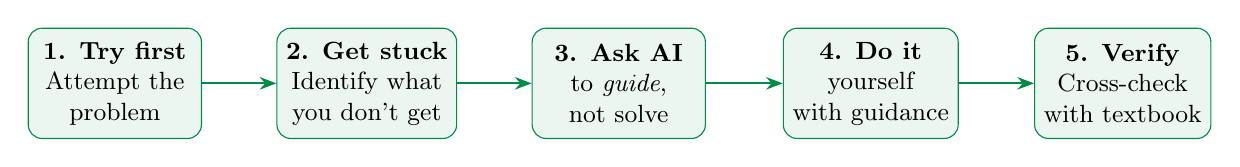
\begin{tikzpicture}[
  box/.style={draw=paramgreen, fill=paramgreen!8, rounded corners=5pt,
              minimum width=2.2cm, minimum height=1.4cm, align=center, font=\small},
  arr/.style={-{Stealth[length=6pt]}, thick, paramgreen}
]
  \node[box] (try) at (0,0) {\textbf{1. Try first}\\Attempt the\\problem};
  \node[box] (stuck) at (3.2,0) {\textbf{2. Get stuck}\\Identify what\\you don't get};
  \node[box] (ask) at (6.4,0) {\textbf{3. Ask AI}\\to \emph{guide},\\not solve};
  \node[box] (do) at (9.6,0) {\textbf{4. Do it}\\yourself\\with guidance};
  \node[box] (ver) at (12.8,0) {\textbf{5. Verify}\\Cross-check\\with textbook};

  \draw[arr] (try) -- (stuck);
  \draw[arr] (stuck) -- (ask);
  \draw[arr] (ask) -- (do);
  \draw[arr] (do) -- (ver);
\end{tikzpicture}
\end{center}

\bigskip
\begin{columns}[T]
\column{0.48\textwidth}
\begin{exampleblock}{The key difference}
\begin{itemize}
  \item ``Help me understand X'' \checkmark
  \item ``Solve X for me'' $\times$
  \item You do the thinking --- AI guides
  \item Learning modes enforce this!
\end{itemize}
\end{exampleblock}

\column{0.48\textwidth}
\begin{exampleblock}{Why this works}
\begin{itemize}
  \item You still struggle (that's learning!)
  \item AI provides scaffolding, not answers
  \item You build real understanding
  \item Knowledge that survives exams
\end{itemize}
\end{exampleblock}
\end{columns}
\end{frame}

% ──────────────────────────────────────────────
\begin{frame}{Prompting for Learning (Part 1)}
\small
\textbf{\color{popblue}Prompts that maximize learning:}

\smallskip
\begin{columns}[T]
\column{0.48\textwidth}
\begin{block}{Guide, don't solve}
\begin{itemize}\setlength\itemsep{0em}
  \item \textit{``Don't give me the answer. Guide me step by step.''}
  \item \textit{``I think the answer is X. Am I right? Where did I go wrong?''}
  \item \textit{``What's wrong with my approach?''}
\end{itemize}
\end{block}

\smallskip
\begin{block}{Explain \& understand}
\begin{itemize}\setlength\itemsep{0em}
  \item \textit{``Explain this using an analogy.''}
  \item \textit{``What's the intuition behind [formula]?''}
  \item \textit{``Why does this work? Not how --- why.''}
\end{itemize}
\end{block}

\column{0.48\textwidth}
\begin{block}{Test yourself}
\begin{itemize}\setlength\itemsep{0em}
  \item \textit{``Quiz me on [topic] --- start easy, then harder.''}
  \item \textit{``Give me 5 practice problems similar to this.''}
  \item \textit{``I studied X. Check if I really understand.''}
\end{itemize}
\end{block}

\smallskip
\begin{block}{Go deeper}
\begin{itemize}\setlength\itemsep{0em}
  \item \textit{``What concept am I missing?''}
  \item \textit{``What are common misconceptions here?''}
\end{itemize}
\end{block}
\end{columns}
\end{frame}

% ──────────────────────────────────────────────
\begin{frame}{Prompting for Learning (Part 2)}
\small
\textbf{\color{popblue}More advanced techniques:}

\smallskip
\begin{columns}[T]
\column{0.48\textwidth}
\begin{block}{Level adjustment}
\begin{itemize}\setlength\itemsep{0em}
  \item \textit{``Explain like I'm a complete beginner.''}
  \item \textit{``Now explain at a graduate level.''}
  \item \textit{``Use only concepts from Calculus 1.''}
\end{itemize}
\end{block}

\smallskip
\begin{block}{Role-based learning}
\begin{itemize}\setlength\itemsep{0em}
  \item \textit{``Act as a [subject] professor --- give me a 5-min lecture on [topic].''}
  \item \textit{``Be my study partner. Let's challenge each other.''}
\end{itemize}
\end{block}

\column{0.48\textwidth}
\begin{block}{Connections \& synthesis}
\begin{itemize}\setlength\itemsep{0em}
  \item \textit{``How does [A] relate to [B]?''}
  \item \textit{``Real-world example of [concept].''}
  \item \textit{``Compare and contrast [X] and [Y].''}
\end{itemize}
\end{block}

\smallskip
\begin{block}{Exam prep}
\begin{itemize}\setlength\itemsep{0em}
  \item \textit{``Study plan for [topic], 2h/day, 5 days.''}
  \item \textit{``Practice exam: 10 questions on ch.\ 5--8.''}
  \item \textit{``Most likely exam questions on [topic]?''}
\end{itemize}
\end{block}
\end{columns}
\end{frame}

% ──────────────────────────────────────────────
\begin{frame}{Combining Tools: A Study Session Workflow}

\begin{center}
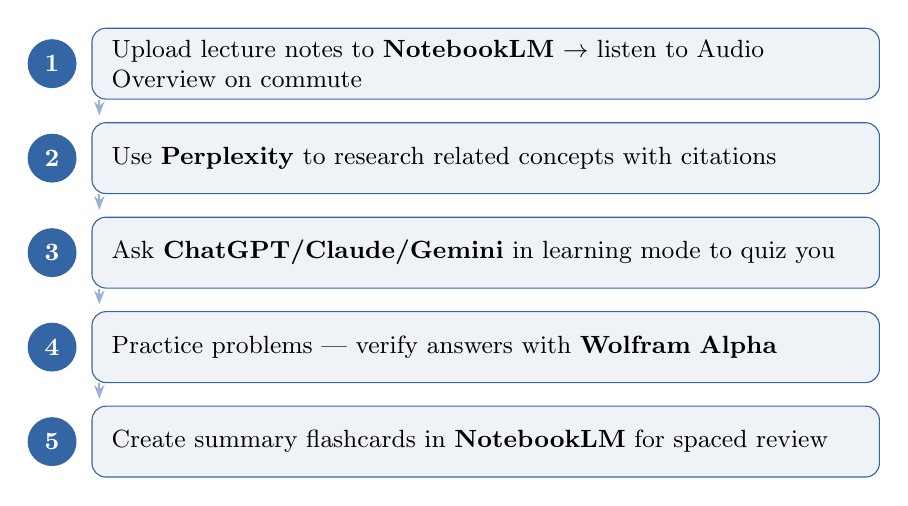
\begin{tikzpicture}[
  sbox/.style={draw=popblue, fill=popblue!8, rounded corners=5pt,
               minimum width=10cm, minimum height=0.9cm, align=left,
               font=\small, text width=9.5cm},
  num/.style={circle, draw=popblue, fill=popblue, text=white,
              minimum size=0.6cm, font=\small\bfseries},
  arr/.style={-{Stealth[length=5pt]}, thick, popblue!50}
]
  \node[num] (n1) at (-5.5, 3.2) {1};
  \node[sbox, anchor=west] (s1) at (-5, 3.2)
    {Upload lecture notes to \textbf{NotebookLM} $\to$ listen to Audio Overview on commute};

  \node[num] (n2) at (-5.5, 2.0) {2};
  \node[sbox, anchor=west] (s2) at (-5, 2.0)
    {Use \textbf{Perplexity} to research related concepts with citations};

  \node[num] (n3) at (-5.5, 0.8) {3};
  \node[sbox, anchor=west] (s3) at (-5, 0.8)
    {Ask \textbf{ChatGPT/Claude/Gemini} in learning mode to quiz you};

  \node[num] (n4) at (-5.5, -0.4) {4};
  \node[sbox, anchor=west] (s4) at (-5, -0.4)
    {Practice problems --- verify answers with \textbf{Wolfram Alpha}};

  \node[num] (n5) at (-5.5, -1.6) {5};
  \node[sbox, anchor=west] (s5) at (-5, -1.6)
    {Create summary flashcards in \textbf{NotebookLM} for spaced review};

  \draw[arr] (s1.south west) ++(0.1,0) -- ++(0,-0.2);
  \draw[arr] (s2.south west) ++(0.1,0) -- ++(0,-0.2);
  \draw[arr] (s3.south west) ++(0.1,0) -- ++(0,-0.2);
  \draw[arr] (s4.south west) ++(0.1,0) -- ++(0,-0.2);
\end{tikzpicture}
\end{center}

\bigskip
\begin{center}
\textbf{Each tool has a strength} --- combine them for maximum learning.
\end{center}
\end{frame}

% ──────────────────────────────────────────────
\begin{frame}{Hallucinations: AI Makes Stuff Up}
\small
\begin{columns}[T]
\column{0.55\textwidth}
\textbf{\color{warnred}What are hallucinations?}
\begin{itemize}\setlength\itemsep{0em}
  \item LLMs generate plausible-sounding but \textbf{wrong} info
  \item They don't ``know'' facts --- they predict likely text
  \item Can invent citations, formulas, historical events
  \item Sounds confident even when completely wrong
\end{itemize}

\smallskip
\textbf{\color{warnred}Educational risks:}
\begin{itemize}\setlength\itemsep{0em}
  \item Learning wrong formulas or definitions
  \item Citing non-existent papers
  \item Building understanding on incorrect foundations
  \item Perplexity: best accuracy, still \textbf{37\% error rate}
\end{itemize}

\column{0.42\textwidth}
\begin{alertblock}{How to protect yourself}
\begin{enumerate}\setlength\itemsep{0em}
  \item \textbf{Always verify} with textbook/professor
  \item Use \textbf{NotebookLM} for source-grounded answers
  \item Use \textbf{Perplexity} for cited research
  \item \textbf{Cross-reference} multiple tools
  \item Be skeptical of confident answers
\end{enumerate}
\end{alertblock}

\smallskip
\begin{exampleblock}{Rule of thumb}
If AI says something surprising, verify before relying on it.
\end{exampleblock}
\end{columns}
\end{frame}

% ──────────────────────────────────────────────
\begin{frame}{Academic Integrity}
\small
\begin{columns}[T]
\column{0.48\textwidth}
\begin{block}{Know your institution's policy}
\begin{itemize}\setlength\itemsep{0em}
  \item AI policies vary \textbf{widely}
  \item Some ban all AI, some encourage it
  \item Some allow for understanding, not submissions
  \item \textbf{Check before using AI for assignments}
\end{itemize}
\end{block}

\smallskip
\begin{exampleblock}{Be transparent}
\begin{itemize}\setlength\itemsep{0em}
  \item Disclose AI use when submitting work
  \item Explain \emph{how} you used it
  \item ``Used Claude to understand, wrote solution myself''
\end{itemize}
\end{exampleblock}

\column{0.48\textwidth}
\begin{block}{The ethical line}
\begin{itemize}\setlength\itemsep{0em}
  \item AI to \textbf{understand} $\neq$ AI to \textbf{cheat}
  \item Tutor: questions, explanations \checkmark
  \item Ghostwriter: generating submissions $\times$
  \item Learning modes keep you on the right side
\end{itemize}
\end{block}

\smallskip
\begin{alertblock}{Remember}
If you can't explain your own work without AI, you didn't learn it --- and it will show on the exam.
\end{alertblock}
\end{columns}
\end{frame}

% ──────────────────────────────────────────────
\begin{frame}{Privacy \& Data}
\small
\begin{columns}[T]
\column{0.48\textwidth}
\textbf{\color{warnred}Be careful what you share:}
\begin{itemize}\setlength\itemsep{0em}
  \item Don't paste personal/sensitive info
  \item Don't share credentials or financial data
  \item Don't upload others' private data
  \item Be cautious with unpublished research
\end{itemize}

\smallskip
\textbf{\color{popblue}Data retention policies differ:}
\begin{itemize}\setlength\itemsep{0em}
  \item ChatGPT: may train on chats (opt out)
  \item Claude: doesn't train by default
  \item Gemini: check settings
  \item NotebookLM: data stays in your account
\end{itemize}

\column{0.48\textwidth}
\begin{exampleblock}{Best practices}
\begin{enumerate}\setlength\itemsep{0em}
  \item Use \textbf{institutional accounts} when available
  \item Check opt-out settings for training
  \item Don't share what you wouldn't post publicly
  \item Use ``temporary chat'' modes
\end{enumerate}
\end{exampleblock}

\smallskip
\textbf{\color{popblue}Institutional offerings:}
\begin{itemize}\setlength\itemsep{0em}
  \item ChatGPT Edu --- enterprise privacy
  \item Claude for Education --- campus deployments
  \item Gemini for Education --- Workspace protections
\end{itemize}
\end{columns}
\end{frame}

% ══════════════════════════════════════════════
% SECTION 5: Wrap-Up
% ══════════════════════════════════════════════
\section{Wrap-Up}

% ──────────────────────────────────────────────
\begin{frame}{Key Takeaways}

\begin{center}
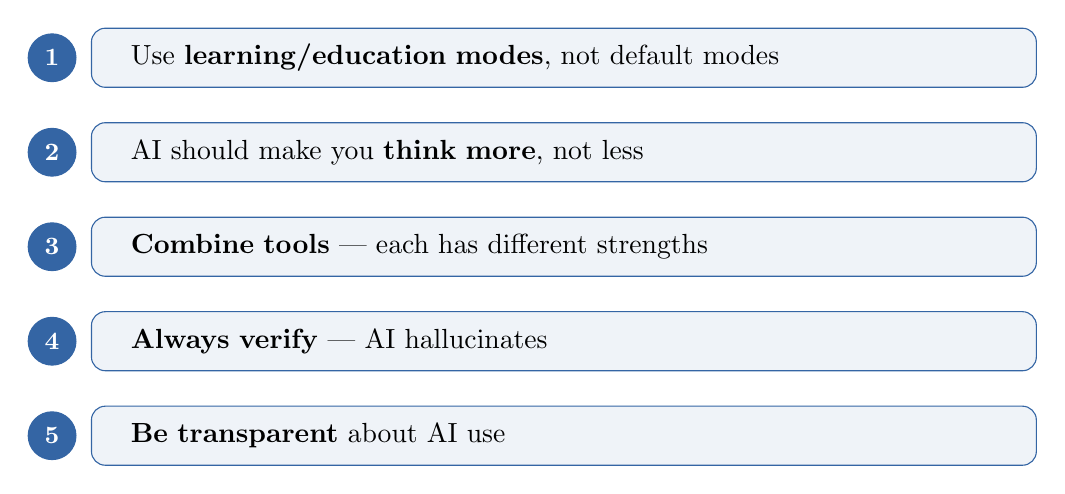
\begin{tikzpicture}[
  take/.style={draw=popblue, fill=popblue!8, rounded corners=5pt,
               minimum width=12cm, minimum height=0.75cm, align=left,
               font=\normalsize, text width=11cm},
  num/.style={circle, draw=popblue, fill=popblue, text=white,
              minimum size=0.55cm, font=\small\bfseries}
]
  \node[num] at (-6.5, 2.4) {1};
  \node[take] at (0, 2.4)
    {Use \textbf{learning/education modes}, not default modes};

  \node[num] at (-6.5, 1.2) {2};
  \node[take] at (0, 1.2)
    {AI should make you \textbf{think more}, not less};

  \node[num] at (-6.5, 0.0) {3};
  \node[take] at (0, 0.0)
    {\textbf{Combine tools} --- each has different strengths};

  \node[num] at (-6.5, -1.2) {4};
  \node[take] at (0, -1.2)
    {\textbf{Always verify} --- AI hallucinates};

  \node[num] at (-6.5, -2.4) {5};
  \node[take] at (0, -2.4)
    {\textbf{Be transparent} about AI use};
\end{tikzpicture}
\end{center}
\end{frame}

% ──────────────────────────────────────────────
\begin{frame}{Free Access for Students}

\begin{center}
\begin{tabular}{@{}l l l@{}}
\toprule
\textbf{Tool} & \textbf{Free access} & \textbf{How} \\
\midrule
ChatGPT & Study Mode on free tier & Sign up at chat.openai.com \\[3pt]
Claude & Free tier available & Sign up at claude.ai \\[3pt]
Gemini & Free for edu institutions & Via Google Workspace for Education \\[3pt]
NotebookLM & Free for everyone & notebooklm.google \\[3pt]
Perplexity Pro & 12 months free & Edu email at perplexity.ai \\[3pt]
GitHub Copilot & Free for students & GitHub Education pack \\[3pt]
Wolfram Alpha & Free basic access & wolframalpha.com \\[3pt]
Khanmigo & \$4/mo (or free via school) & khanmigo.ai \\[3pt]
Grammarly & Free tier available & grammarly.com \\[3pt]
Gamma AI & Free tier available & gamma.app \\
\bottomrule
\end{tabular}
\end{center}

\bigskip
\begin{center}
\textbf{Most of these tools are free or have generous student programs.}\\
You have no excuse not to try them!
\end{center}
\end{frame}

% ──────────────────────────────────────────────
\begin{frame}{Resources \& Links}

\begin{columns}[T]
\column{0.48\textwidth}
\textbf{\color{popblue}The Big Three:}
\begin{itemize}
  \item ChatGPT: \texttt{chat.openai.com}
  \item Claude: \texttt{claude.ai}
  \item Gemini: \texttt{gemini.google.com}
\end{itemize}

\bigskip
\textbf{\color{paramgreen}Study \& Research:}
\begin{itemize}
  \item NotebookLM: \texttt{notebooklm.google}
  \item Perplexity: \texttt{perplexity.ai}
  \item Khanmigo: \texttt{khanmigo.ai}
  \item Wolfram Alpha: \texttt{wolframalpha.com}
\end{itemize}

\column{0.48\textwidth}
\textbf{\color{orange1}Coding:}
\begin{itemize}
  \item GitHub Copilot: \texttt{github.com/features/copilot}
  \item GitHub Education: \texttt{education.github.com}
  \item Replit: \texttt{replit.com}
\end{itemize}

\bigskip
\textbf{\color{violet1}Writing \& Productivity:}
\begin{itemize}
  \item Grammarly: \texttt{grammarly.com}
  \item Notion AI: \texttt{notion.so}
  \item Gamma AI: \texttt{gamma.app}
\end{itemize}
\end{columns}
\end{frame}

% ──────────────────────────────────────────────
\begin{frame}{}

\begin{center}
\vspace{2cm}
{\Huge\color{popblue}\textbf{Questions?}}

\vspace{1.5cm}
{\large Use AI to learn better --- not to learn less.}
\end{center}
\end{frame}

\end{document}
